\chapter{Domains and Coordinate Systems}\label{Chp:ref:coordinates}

If the region of interest is reasonably small a flat Earth can be assumed. In this case
it is sufficient to use a Cartesian domain\index{Cartesian Domain} $\Omega$ in the form
\begin{equation} \label{REF:EQU:INTRO 8}
\Omega = [x^{min}_0, x^{max}_0] \times
 [x^{min}_1, x^{max}_1] \times
 [x^{min}_2, x^{max}_2] 
\end{equation} 
and use the 
where $x_0$ represents the easting, $x_1$ the northing and $x_2$ the altitude in meters, see Figure~\ref{fig:cartesianDomain}.
It is assumed that data are given is longitude-latitude coordinates which are projected using the   
Universal Transverse Mercator (UTM) coordinate system\footnote{See
    e.g. \url{http://en.wikipedia.org/wiki/Universal_Transverse_Mercator_coordinate_system}.}. 
In this way, all three coordinates can be given in meters with minimal
distortion when visualizing the domain.
The origin in vertical direction (altitude 0) corresponds to sea level.
For some cases, typically if no sufficient data are available, it is appropriate 
to add buffer zones in all dimensions. It can be appropriate to add lateral buffer zones if the 
extend of the area covered by the available data is small. 
Figure~\ref{fig:cartesianDomain} depicts these as areas shaded in red (padding
area) and blue (air buffer).
While the inversion results contain values for the entire domain the buffer zone
should be disregarded when performing any analysis.
In other words, only the region labeled \emph{data area} in
Figure~\ref{fig:cartesianDomain} contains useful information.
Both the thickness of the air layer and the amount of padding in the $x_0$/$x_1$
dimension is configurable when setting up an inversion.

\begin{figure}[ht]
    \centering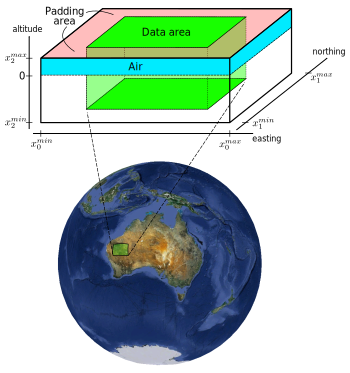
\includegraphics{cartesian}
    \caption{Illustration of domain extents, mapping and padding area}
    \label{fig:cartesianDomain}
\end{figure}

\begin{figure}[t]
    \centering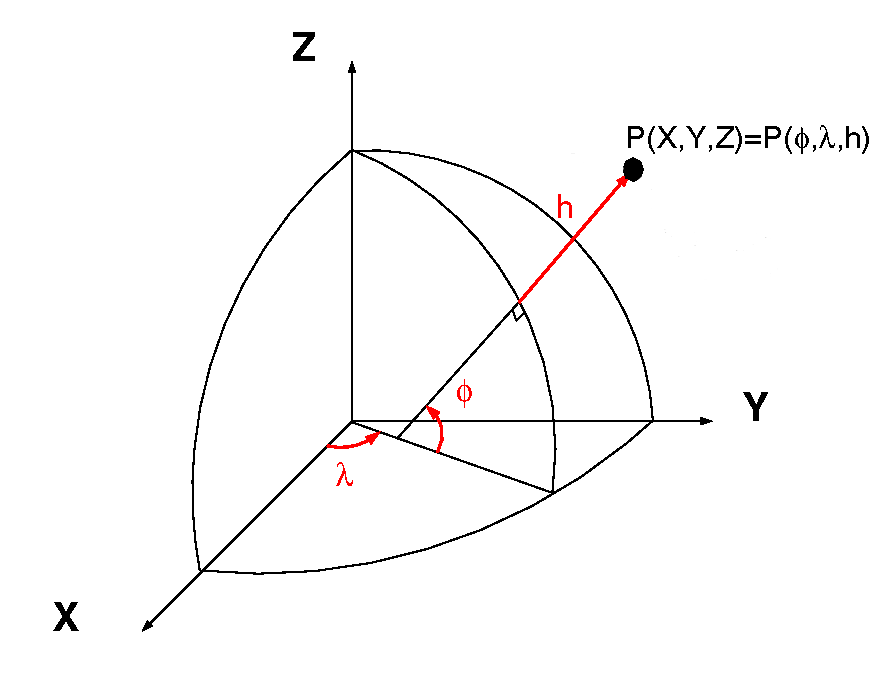
\includegraphics[width=0.7\textwidth]{geosphir}
    \caption{Geodetic coordinates  $( \lambda, \phi,h)$ of a point $P$ with 
cooridnates $(X,Y,Z)=(x_0,x_1,x_2)$ (thanks to the National Geodetic Survey of the National Oceanic and Atmospheric Administration (NOAA), 
see \url{http://www.ngs.noaa.gov/)}.
}
    \label{fig:geodeticDomain}
\end{figure}
For larger areas on the Earth surface it is essential consider the curvature of the region of interest. For this case 
it is appropriate to describe the domain of interest using longitude, latitude and height above Earth surface to describe 
the domain of interest. We use the geodetic coordinates (see Figure~\ref{fig:geodeticDomain}) where the location of a point 
is described by its geodetic latitude $\phi$ (in $deg$), longitude 
$\lambda$ (in $deg$) and geodetic height $h$ (in $km$)~\cite{Featherstone2008a} where we assume
\begin{equation}
  -90^o \le \phi \le 90^o \mbox{ and } -180^o \le \lambda \le -180^o \;.
\end{equation} 
In the following we refer to the $(\phi, \lambda, h)$ as the Geodetic Coordinate system\index{geodetic coordinates}.
In practice we will be interested in a subregion $\Omega$ which is given by the coordinate region   
\begin{equation} \label{REF:EQU:INTRO 8b}
\widehat{\Omega} = 
 [\lambda^{min}, \lambda^{max}] \times [\phi^{min}, \phi^{max}] \times
 [h^{min}, h^{max}] 
\end{equation} 
The Cartesian coordinates $(x_0,x_1,x_2)$ of a point are given as 
\begin{equation}
\begin{array}{rcll}
   x_0 & = &  (N + f_{h}  \cdot  h) & \cdot \cos(f_{a} \cdot  \phi) \cdot  \cos(f_{a} \cdot  \lambda) \\
   x_1 & = &  (N + f_{h}  \cdot  h) & \cdot  \cos(f_{a} \cdot  \phi) \cdot  \sin(f_{a} \cdot  \lambda) \\
   x_2 & = &  (N \cdot (1-e^2) + f_{h}  \cdot  h ) & \cdot  \sin(f_{a} \cdot  \phi)\\
\end{array}
\label{equ:geodetic:1}
\end{equation} 
where $N$ is given as 
\begin{equation}
 N = \frac{a}{\sqrt{1- e^2 \cdot \sin^2(f_{a} \cdot  \phi) }}
\label{equ:geodetic:2}
\end{equation}
with the semi major axis length $a$ and $b$ ($ a \ge b$), and the eccentricity 
\begin{equation} \label{equ:ref:coordinates:100}
e = \sqrt{2f - f^2} \mbox{ with flattening } f = 1-\frac{b}{a} \ge 0
\end{equation}
The factors $f_{a}$ and $f_{h}$ consider the change of units from 
$deg$ to $rad$ and $km$ to $m$, respectively.
Notice that the surface of the ellipsoid (Earth) is described by the case $h=0$.  Table~\ref{REF:FIG:REF:10}
shows values for  flattening semi-major axis for the major reference systems of the Earth.

\begin{table}
\begin{center}
\begin{tabular}{c|lll}
Ellipsoid reference & Semi-major axis a & Semi-minor axis b & Inverse flattening (1/f)\\
\hline
GRS 80 & 6 378 137.0 m & 6 356 752.314 140 m & 298.257 222 101\\
WGS 84 & 6 378 137.0 m & 6 356 752.314 245 m & 298.257 223 563
\end{tabular}
\end{center}
\caption{Geodetic Reference Systems of the Earth}\label{REF:FIG:REF:10}
\end{table}

We need to translate any object from the Cartesian coordinates $(x_i)$ in terms of Geodetic Coordinate system
$(\phi, \lambda, h)$. In the following indexes running through $(\phi, \lambda, h)$ are denoted by little Greek letters $\alpha$, 
$\beta$
to separate them from indexes running through the components of the Cartesian coordinates system in little Latin letters.
With this convection the derivative of a function $g$ with respect to the Geodetic coordinates which is given as
\begin{equation}
\begin{array}{rcl}
  g_{,\lambda} & =  & g_{,0} \cdot x_{0,\lambda} + g_{,1} \cdot x_{1,\lambda} + g_{,2} \cdot x_{2,\lambda} \\  
  g_{,\phi} & =  & g_{,0} \cdot x_{0,\phi} + g_{,1} \cdot x_{1,\phi} + g_{,2} \cdot x_{2,\phi} \\
  g_{,h} & =  & g_{,0} \cdot x_{0,h} + g_{,1} \cdot x_{1,h} + g_{,2} \cdot x_{2,h} \\
\end{array}
\end{equation}
via chain rule can be written in the compact form 
\begin{equation}
  g_{,\alpha}   =    g_{,i} \cdot x_{i,\alpha} 
\end{equation}
with
\begin{equation}
 x_{i,\alpha}
= 
\left[
\begin{array}{ccc}
-  R_N \cdot \cos(f_{a} \cdot  \phi) \cdot  \sin(f_{a} \cdot  \lambda) & - R_M \cdot \sin(f_{a} \cdot  \phi) \cdot  \cos(f_{a} \cdot  \lambda) &  f_{h}  \cdot  \cos(f_{a} \cdot  \phi) \cdot  \cos(f_{a} \cdot  \lambda)  \\
 R_N  \cdot  \cos(f_{a} \cdot  \phi) \cdot  \cos(f_{a} \cdot  \lambda) &   -  R_M \cdot  \sin(f_{a} \cdot  \phi) \cdot  \sin(f_{a} \cdot  \lambda) &   f_{h}  \cdot  \cos(f_{a} \cdot  \phi) \cdot  \sin(f_{a} \cdot  \lambda) \\
 0 &  R_M  \cdot  \cos(f_{a} \cdot  \phi) &    f_{h}  \cdot  \sin(f_{a} \cdot  \phi) \\
\end{array}
\right]
\end{equation}
with 
\begin{equation}
R_M = f_{a}  \cdot (M + f_{h}  \cdot h) \mbox{ and }
R_N = f_{a}  \cdot  (N + f_{h}  \cdot h) 
\label{equ:geodetic:5}
\end{equation}
and 
\begin{equation}
 M = \frac{a \cdot  (1-e^2) }{(1- e^2 \cdot \sin^2(f_{a} \cdot  \phi))^{\frac{3}{2}}}
\label{equ:geodetic:5b}
\end{equation}
With the coordinate vectors $(u_{\alpha})$ defined as 
\begin{equation}
u_{i \alpha} = d_{\alpha \alpha} x_{i,\alpha}
\end{equation}
and scaling factors 
\begin{equation}
d_{\lambda \lambda} =  \frac{1}{f_{a} \cdot (N + f_{h} \cdot h) \cdot \cos(f_{a} \cdot  \phi)}  \; , 
d_{\phi \phi} = \frac{1}{f_{a} \cdot (M + f_{h} \cdot h)} \mbox{ and }
d_{h h} = \frac{1}{f_{h}}
\end{equation}
we get 
\begin{equation}
g_{,\alpha}   =    g_{,i} u_{i \alpha} \frac{1}{d_{\alpha \alpha}} 
\end{equation}
With the fact that 
\begin{equation}
 u_{i \alpha} u_{j \alpha} = \delta_{ij} \mbox{ and }  u_{i \alpha} u_{i \beta} = \delta_{\alpha \beta}
\end{equation}
\begin{equation}
g_{,i} = d_{\alpha \alpha} g_{,\alpha}  u_{i \alpha} 
\end{equation}
or 
\begin{equation}
g_{,i} = 
\frac{1}{f_{a} \cdot (N + f_{h} \cdot h) \cdot \cos(f_{a} \cdot  \phi) }  g_{,\lambda}  u_{i \lambda} +
\frac{1}{f_{a} \cdot (M + f_{h} \cdot h)}   g_{,\phi}  u_{i \phi} + 
\frac{1}{f_{h}}  u_{i h} 
\end{equation} 
Moreover for integrals we get by substitution rule 
\begin{equation}
dx_0 \; dx_1  \;  dx_2 =\det((x_{i,\alpha}))  \;  d \phi  \;   d\lambda   \;  dh = v \;  d \phi  \;   d\lambda   \;  dh
\end{equation} 
with  $v= \frac{1}{d_{\phi \phi} d_{\lambda \lambda} d_{h h}} =
f_{a}^2 f_{h} (M + f_{h} \cdot h) (N + f_{h} \cdot h) \cdot \cos(f_{a} \cdot  \phi) 
$.
Notice that for a spherical Earth $e=0$ for which $M=N$ is the radius of the Earth and $M+h$ is the distance from
the center \footnote{It is useful to keep in mind that
for the Cartesian cooridnate system $(x_0, x_1, x_2) = (\phi, \lambda, h)$ and $v=1$ and $d_{\alpha \alpha}=1$}. 

\section{Reference Systems}\label{sec:ref:reference systems}
The \class{ReferenceSystem} is an identifier for a coordinate system which is used to define a 
transformation from a rectangular domain $\widehat{\Omega}$ to a subregion at and around the surface of the Earth. 
Although the terminology can be applied to a any orthogonal coordinate system in practice
we have two relevant cases, namely the case the Cartesian coordinate system where no coordinate transformation
is applied ($\widehat{\Omega}= \widehat{\Omega}$) and a Geodetic coordinate system as described above. 
The two class \class{CartesianReferenceSystem} and \class{GeodeticReferenceSystem} as described in the 
next subsection implement a \class{ReferenceSystem}.

\subsection{Cartesian Reference Systems}
\begin{classdesc}{CartesianReferenceSystem}{}
the Cartesian reference coordinate system.
\end{classdesc}

\begin{methoddesc}[GeodeticReferenceSystem]{isCartesian}{}
returns \True 
\end{methoddesc}


\begin{methoddesc}[CartesianReferenceSystem]{isTheSame}{other}
test if \member{other} is also the Cartesian reference coordinate system
\end{methoddesc}


\begin{methoddesc}[CartesianReferenceSystem]{createTransformation}{domain}
creates the appropriate coordinate transformation \class{CartesianCoordinateTransformation} on a given \member{domain}
from the reference coordinate system.
\end{methoddesc}


\subsection{Geodetic Reference Systems}

\begin{classdesc}{GeodeticReferenceSystem}{
  \optional{ a=6378137.0} 
  \optional{, f=1/298.257223563} 
  \optional{, name="WGS84"}
}
initializes a geodetic reference system. 
\member{a} is the length of the semi-major axis in meter.
\member{f} is the flattening, see equation~\ref{equ:ref:coordinates:100}.  
\member{name} sets the name for the reference system 
\end{classdesc}


\begin{methoddesc}[GeodeticReferenceSystem]{isCartesian}{}
returns \False 
\end{methoddesc}


\begin{methoddesc}[GeodeticReferenceSystem]{getSemiMajorAxis}{}
returns the length of semi major axis
\end{methoddesc}

\begin{methoddesc}[GeodeticReferenceSystem]{getSemiMinorAxis}{}
returns the length of semi minor axis
\end{methoddesc}

\begin{methoddesc}[GeodeticReferenceSystem]{getFlattening}{}
returns the flattening
\end{methoddesc}


\begin{methoddesc}[GeodeticReferenceSystem]{isTheSame}{other}
test if \member{other} defines the same reference coordinate system.
\end{methoddesc}


\begin{methoddesc}[GeodeticReferenceSystem]{createTransformation}{domain}
creates the appropriate coordinate transformation \class{GeodeticReferenceSystem}  on a given \member{domain}
from the reference coordinate system.
\end{methoddesc}

\subsection{Short Cuts} 
And some shorts cuts for some standart reference systems:
\begin{funcdesc}{SphericalReferenceSystem}{\optional{R=6378137.0}}
returns the \class{GeodeticReferenceSystem} of a sphere of radius \member{R} in meters.
\end{funcdesc}

\begin{funcdesc}{WGS84ReferenceSystem}{}
returns the \class{GeodeticReferenceSystem} for the WGS84 Ellipsoid, see Table~\ref{REF:FIG:REF:10}.
\end{funcdesc}

\begin{funcdesc}{GRS80ReferenceSystem}{}
returns the \class{GeodeticReferenceSystem} for the GRS80 Ellipsoid, see Table~\ref{REF:FIG:REF:10}.
\end{funcdesc}

\section{Coordinate Transformation}\label{sec:ref:trafo}
A coordinate transformation defines a transformation of a reference domain $\widehat{\Omega}$ using
a coordinate reference system~\footnote{In general any orthogonal coordinate transformation can be supported
by building subclasses of the \class{SpatialCoordinateTransformation}}. The following script shows the usage:
\begin{python}
from escript.ripley import Brick
domain=Brick(10,10, 30, l0=[-35.,-34.], l1=[148.,149], l2=[-40.,40.])
trafo=GeodeticCoordinateTransformation(domain, WGS84ReferenceSystem())
\end{python}
or in a more generic form:
\begin{python}
from escript.ripley import Brick
ref=WGS84ReferenceSystem()
domain=Brick(10,10, 30, l0=[-35.,-34.], l1=[148.,149], l2=[-40.,40])
trafo=ref.createTransformation(domain)
\end{python}
Notice that the coordinate ranges for latitude (\member{l0}) and 
longitude (\member{l1}) are given in degree amd
the range for height $h$ above surface (\member{l2}) in $km$.
The \member{trafo} objects provides now access to the volume factor $v$ and the scaling factors $d_{\alpha, \alpha}$.   
The class \\ \class{GeodeticCoordinateTransformation} has the following interface:
\begin{classdesc}{GeodeticCoordinateTransformation}{domain \optional{, reference=WGS84ReferenceSystem()}}
defines a geodetic coordinate transformation with \member{domain} ($=\widehat{\Omega}$) 
using the reference coordinate system \member{reference}. 
Argument \member{domain} needs to be an \escript \class{Domain} object.
\member{reference}, if present, needs to be a \class{GeodeticReferenceSystem} class object.
\end{classdesc}


\begin{methoddesc}[GeodeticCoordinateTransformation]{isTheSame}{other}
tests of \member{other} defines the same coordinate transformation, i.e. uses the same reference system and the same domain.
\end{methoddesc}


\begin{methoddesc}[GeodeticCoordinateTransformation]{isCartesian}{}
returns \False.
\end{methoddesc}

\begin{methoddesc}[GeodeticCoordinateTransformation]{getDomain}{}
returns the domain of the coordinate transformation.
\end{methoddesc}


\begin{methoddesc}[GeodeticCoordinateTransformation]{getReferenceSystem}{}
returns the reference system used to define the coordinate transformation
\end{methoddesc}


\begin{methoddesc}[GeodeticCoordinateTransformation]{getVolumeFactor}{}
returns the volume factor for the coordinate transformation $v$.
\end{methoddesc}


\begin{methoddesc}[GeodeticCoordinateTransformation]{getScalingFactors}{}
returns the scaling factors $d_{\alpha, \alpha}$.
\end{methoddesc}

\begin{methoddesc}[GeodeticCoordinateTransformation]{getGradient}{u}
return the gradient of scalar \member{u} along the axis of
reference coordinate system.
\end{methoddesc}

\subsection{Cartesian Transformation}
In order to be able to use Cartesian coordinates  within \downunder in the same way like geodetic coordinates 
one can use the class \class{CartesianCoordinateTransformation}.  It defines the same interface 
like the 
\class{GeodeticCoordinateTransformation} class:
\begin{python}
from escript.ripley import Brick
ref=CartesianReferenceSystem()
domain=Brick(10,10, 30, l0=[0.,10000], l1=[0.,10000], l2=[-40000.,40000])
trafo=ref.createTransformation(domain)
\end{python}
Notice that the coordinate ranges for North-South extend (\member{l0}) and 
East_West extend (\member{l1}) and height above ground level (\member{l2})  are given in meters now.

\begin{classdesc}{CartesianCoordinateTransformation}{domain}
defines a Cartesian coordinate transformation with domain \member{domain}. In fact no coordinate transformation is
transformed.  
\end{classdesc}


\begin{methoddesc}[CartesianCoordinateTransformation]{isTheSame}{other}
tests of \member{other} defines the same coordinate transformation, i.e. uses the same reference system and the same domain.
\end{methoddesc}


\begin{methoddesc}[CartesianCoordinateTransformation]{isCartesian}{}
returns \True.
\end{methoddesc}

\begin{methoddesc}[CartesianCoordinateTransformation]{getDomain}{}
returns the domain of the coordinate transformation.
\end{methoddesc}


\begin{methoddesc}[CartesianCoordinateTransformation]{getReferenceSystem}{}
returns the reference system used to define the coordinate transformation (an instance of \class{CartesianReferenceSystem})
\end{methoddesc}


\begin{methoddesc}[CartesianCoordinateTransformation]{getVolumeFactor}{}
returns the volume factor for the coordinate transformation $v$ ($=1$).
\end{methoddesc}


\begin{methoddesc}[CartesianCoordinateTransformation]{getScalingFactors}{}
returns the scaling factors $d_{\alpha \alpha}$ ($=1$).
\end{methoddesc}

\begin{methoddesc}[CartesianCoordinateTransformation]{getGradient}{u}
return the gradient of scalar \member{u} along the axis of
reference coordinate system.
\end{methoddesc}
